\large

\section{Hadronically decaying $\tau$ lepton}
\label{sec:rec:tau}
With a mass of 1.777 GeV and a proper decay length
of 87 $\mu$m~\cite{PDG}, tau leptons decay either leptonically
($\tau_{lep} \rightarrow \ell \nu \ell \nu \tau$, $\ell  = e, \mu$ ) 
or hadronically ($\tau_{had} \rightarrow$ hadrons $\nu_{\tau}$) 
and do so typically before reaching active
regions of the \hbox{ATLAS} detector. 
The leptonically decaying $\tau_{lep}$ is simply reconstructed
as either an electron or muon, with the netrinos contributing 
to the real component of the \met. 
On the other hand, the hadronically decaying $\tau_{tau}$ 
can be identified via their decay products. 
The hadronic tau lepton decays represent 65\% of all possible decay modes~\cite{PDG}. 
In these decay modes, the hadronic decay products are 
one or three charged pions in 72\% and 22\% of all cases, respectively. 
Charged kaons are present in the 
majority of the remaining hadronic decays. 
In 78\% of all hadronic decays, up to one associated neutral pion is
also produced. 
This results in an experimental signature of a collimated
calorimeter shower with either one or three associated tracks (\textit{prongs}).
The neutral and charged hadrons stemming from 
the tau lepton decay make up the visible
decay products of the tau lepton, 
and are in the following referred to as \tauhadvis.

\subsection{Reconstruction}
The \tauhadvis\ candidates are
seeded by jets formed using the anti-$k_t$ algorithm,
with a jet-size parameter $R$ = 0.4. 
For events with multiple interactions, the chosen primary may not be the
one where the tau lepton originated. 
Here the \textit{tau vertex association} algorithm is used with 
all tau candidates tracks within a region of $\Delta R$ < 0.2 
around the jet seed direction as input. 
The \pt\ of these tracks is summed and the 
primary vertex candidate to which the largest fraction
of the \pt\ sum is matched to is chosen as the tau vertex~\cite{ATLAS-CONF-2014-018}.

Tracks are associated with the \tauhadvis\ if they are
in the \textit{core} region $\Delta R$ < 0.2 
around the \tauhadvis\ direction and 
satisfy the following criteria: \pt\ > 1 GeV, 
at least two associated hits in the pixel layers of the inner detector, 
and at least seven hits in total in the pixel and the SCT layers. 
Furthermore, requirements are imposed on 
the distance of closest approach of the track to the vertex
in the transverse plane, $|d_0|$ < 1.0 mm, and
longitudinally, $|z_0 sin\theta|$ < 1.5 mm. 
Tracks in the \textit{isolation} region 0.2 < $\Delta R$ < 0.4 
are used for the calculation of identification variables 
and are required to satisfy the same selection criteria.
% A set of boosted decision trees (BDTs) is used to classify all 
% tracks within $\Delta R$ = 0.4 of the \tauhadvis\ axis 
% into core and isolation tracks, depending on their \pt, 
% the number of hits in the tracking detectors 
% as well as their transverse and
% longitudinal impact parameters with respect to the tau vertex. 
The number of tracks (prongs) is susceptible
to underestimation due to tracking inefficiency, 
or overestimation due to tracks from
photon conversions passing the track selection criteria.

\subsection{Identification}
The \tauhadvis\ reconstruction algorithm alone provides 
no discrimination against other particles that result in
jet-like signatures in the detector. 
Therefore, dedicated algorithms are used to identify hadronic tau lepton
decays. Here, a recurrent neural network (RNN) classifier 
is used as described in Ref.~\cite{ATL-PHYS-PUB-2019-033}.
The RNN uses a combination of low-level input variables 
for individual tracks and clusters that are associated 
to the \tauhadvis\ candidate as well as several 
high-level observables calculated from track and
calorimeter quantities.
Due to the distinct signatures of 1- and 3-prong $\tau_{had}$ decays, 
the \tauhadvis\ identification is split into dedicated
algorithms for 1- and 3-prong \tauhadvis. 
Four working points with increasing background rejection 
(\textit{Very loose}, \textit{Loose}, \textit{Medium}
and \textit{Tight}) are defined to be used by physics analyses.
The corresponding signal selection efficiencies and
rejection powers are given in Table~\ref{tab:tauID}.

\begin{table}[tb!]
    \begin{center}{\large    
    \resizebox{0.9\textwidth}{!}{\begin{tabular}{llllllll}
    \toprule
     & \multicolumn{2}{l}{Signal efficiency} &\multicolumn{2}{l}{Background rejection BDT}  &\multicolumn{2}{l}{Background rejection RNN}  \\
    Working point& 1-prong & 3-prong & 1-prong & 3-prong & 1-prong & 3-prong\\
    \midrule
    Tight & 60\% & 45\% &   40      &400   & 70 &700 \\
    Medium & 75\% & 60\% &  20      &150   & 35 &240 \\
    Loose & 85\% & 75\% &   12      &61    & 21& 90 \\
    Very loose & 95\% & 95\% &   5.3 &11.2  & 9.9& 16 \\
    \midrule
    \bottomrule
    \end{tabular}}}
    \end{center}
    \caption
    { List of defined working points with fixed true \tauhadvis\ selection 
    efficiencies and the corresponding background
    rejection factors for misidentified \tauhadvis\ in dijet events 
    for the BDT and RNN classifiers. 
    Table reproduced from Ref.~\cite{ATL-PHYS-PUB-2019-033}.
    \protect\label{tab:tauID}}
    \end{table}
    


Compared to the ID that was used in the analysis of the 36.1 fb$^{-1}$ data~\cite{HIGG-2016-16},
which was based on a boosted decision tree, 
the RNN tau-ID shows better performance 
and allows to move to a looser WP gaining increased efficiency 
(about 24\% and 11\% in case of two $\tau_{had}$ and 
one $\tau_{had}$ in the final state, respectively) 
without losing jet rejection, as shown in Figure~\ref{fig:RNNtau}. 

Selected \tauhadvis\ candidates in the analysis are required to have 
\pt\ > 20 GeV, $|\eta|$ < 2.5, with candidates in the barrel-endcap 
transition region of the calorimeter (1.37 < $|\eta|$ < 1.52) vetoed 
due to poor detector instrumentation in this region, 
one or three tracks, unit charge, and to pass the `loose' $\tau_{had}$--ID working point.
The loose WP corresponds to 85\% efficiency for 1-prong 
and 75\% efficiency for 3-prong (the efficiency is
flat in \pt\ by definition).
\begin{figure}[bth]
	\begin{centering}	
	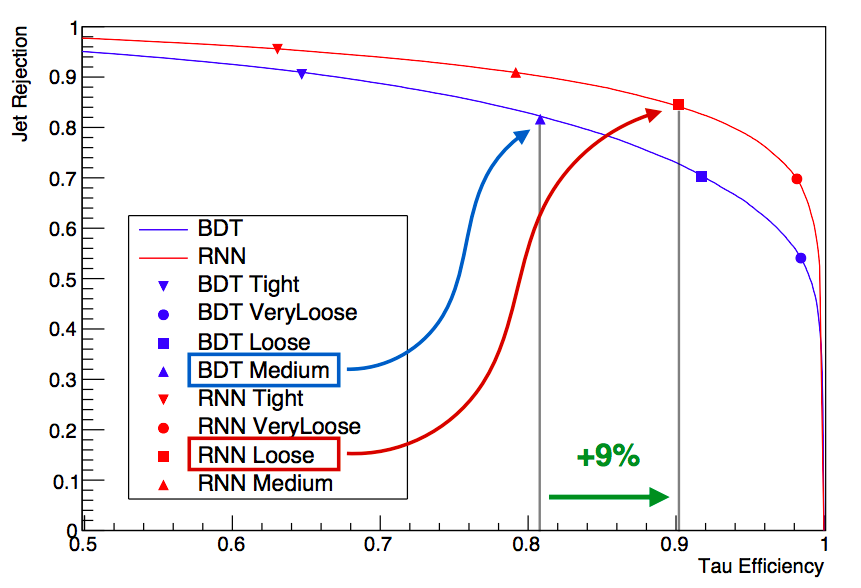
\includegraphics[width=.9\textwidth]{Reconstruction/plots/tauRNN.png}
	\caption{Jet rejection and tau efficiency of tau candidate, 
    measured in $\gamma^* \rightarrow \tau\tau$ sample for RNN-ID~\cite{ATL-PHYS-PUB-2019-033}
    and $Z/\gamma^* \rightarrow \tau\tau$ sample for BDT-ID~\cite{ATL-PHYS-PUB-2015-045}.
    Jet rejection represents the probability of a jet 
    not originating from a tau lepton being rejected 
    by the identification algorithm.
    The green arrow indicates the increase in tau efficiency.
    Figure}
	\label{fig:RNNtau}
	\end{centering}
\end{figure}

Additional rejection of \tauhadvis\ candidates originating 
from electrons is provided by a BDT employing track
and shower shape information. The `loose' working point is used
for the analysis presented in Chapter~\ref{sec:search for dihiggs}, 
corresponding to a selection efficiency
of about 95\% efficiency for true \tauhadvis~\cite{ATLAS-CONF-2017-029}.
% Studies on the comparison between the BDT 
% (used in the previous round of the analysis) and RNN $\tau_{had}$--IDs
% and on the choice of the working point are reported in Appendix C.3. 


\section{Missing transverse energy}
As defined in section~\ref{eq:MET}, the $\vec{E_T}^{miss}$ is given 
as
$\vec{E_T}^{miss}=-\sum_i \vec{p_{T_i}}$
,
which is the negative vector sum of transverse momentum collected from the 
detector, from which one or more ``invisible'' particle(s) can be inferred.
The reconstruction of $\vec{E_T}^{miss}$ is comprised of two contributions~\cite{MET2018},
within the region of $|\eta|$ < 4.9. 
The first one is from \textit{hard-event} signals, combining 
information from fully reconstructed and calibrated 
physics objects, i.e.\ electrons, muons, photons, jets,
hadronically decaying $\tau$-leptons and jets. 
The second one is from the \textit{soft-event} signals, consisting of 
reconstructed charged-particle tracks associated with the hard-scatter
vertex but with no physics objects.
Hence, the \MET\ is calculated as:
\[ E^{miss}_T = - \sum_{\substack{\text{selected}\\ \text{electrons}}} p^e_T 
- \sum_{\substack{\text{accepted} \\  \text{photons}}} p^{\gamma}_T   
- \sum_{\substack{\text{accepted} \\  \text{$\tau$-leptons}}} p^{\tau_{had}}_T 
- \sum_{\substack{\text{selected} \\  \text{muons}}} p^{\mu}_T 
- \sum_{\substack{\text{accepted} \\  \text{jets}}} p^{jet}_T 
- \sum_{\substack{\text{unused}\\ \text{tracks}}} p^{track}_T
\].


% A deviation of the total transverse momentum from zero can
A non-zero \MET\ suggests
the existence of a non-interacting particle.
In the SM, the only particle that does
not deposit energy in the detector are neutrinos, 
as they are weakly interacting leptons
which do not undergo the strong or electromagnetic forces.
Nevertheless, some BSM theories predict
the existence of additional weakly-interacting particles.

\section{Overlap removal}
After the event is reconstructed, an overlap-removal procedure is applied 
to resolve ambiguities when a physical object is reconstructed as multiple 
particles in the \hbox{ATLAS} detector. The angular distance $\Delta R$ is used 
to measure the overlap of two reconstructed objects.
Overlaps between most of the detector objects used in the analysis are resolved 
by using the standard overlap removal tools AssociationUtils~\cite{ORTool}, 
with analysis specific procedure for 
the reconstructed \tauhadvis\, anti-\tauhadvis\ objects and jets.
The step-by-step procedure that is used to resolve ambiguities in the 
reconstructed objects is summarised in  the following:
 \begin{itemize}
     \item  $e_1$--$e_2$: For two electrons $e_1$ and $e_2$ in an event,  
     reject $e_1$ if both electrons share the track and $p_{T1}$ < $p_{T2}$
    \item  \tauhadvis\--$e$: Reject \tauhadvis\ if $\Delta R$ < 0.2 
    % and   $e$ passes \hbox{DFCommonElectronsLHLoose}
    \item  \tauhadvis\--$\mu$: Reject \tauhadvis\ if $\Delta R$ < 0.2:
     \\ Case 1 (\tauhadvis\ $p_T$ > 50GeV): $p_T$, $\mu$ > 2GeV and combined muon
     \\ Case 2 (\tauhadvis\ $p_T$ $\leq$ 50GeV): $p_T$, $\mu$ > 2GeV
    \item  $\mu$--$e$: Reject $\mu$ if calo-muon and shared ID track
    \item  $e$--$\mu$: Reject $e$ if shared ID track
    \item  jet--$e$: Reject jet if $\Delta R$ < 0.2
    \item  $e$--jet: Reject $e$ if $\Delta R$ < 0.4
    \item  jet--$\mu$: Reject jet if $N_{track}$ < 3 ($p_{T}^{track}$ > 500MeV), and $\Delta R$ < 0.2
    \item  $\mu$--jet: Reject $\mu$ if $\Delta R$ < 0.4
 \end{itemize}
 Additionally, an analysis-specific overlap-removal procedure for \tauhadvis\, 
 anti-\tauhadvis\ and jets is implemented:
\begin{itemize}
    \item jet--\tauhadvis\: Reject jet if $\Delta R$ < 0.2
    \item anti--\tauhadvis\--jet: Reject anti--$\tau_{had}$ if jet is $b$-tagged and $\Delta R$ < 0.2
    \item jet--anti--\tauhadvis\: Reject jet if $\Delta R$ < 0.2
\end{itemize}
 This establishes the following priority: \tauhadvis\ > $b$-tagged jet > anti-\tauhadvis\ > un-tagged jet.
%  Another priority, $b$-tagged jet > \tauhadvis\ > anti-\tauhadvis\ > un-tagged jet, was investigated as an alternative
%  but found to reduce signal acceptance in the 2-tag region significantly due to limited $\tau_{had}$ rejection of the
%  DL1r $b$-tagging algorithm at the 77\% working point. With the alternative priority the signal acceptance is
%  reduced by about 8\% (13\%) in $\tau_{lep}$$\tau_{had}$ ($\tau_{had}$$\tau_{had}$).
\label{sec:overlap}

